% Copyright 2007 by Till Tantau
%
% This file may be distributed and/or modified
%
% 1. under the LaTeX Project Public License and/or
% 2. under the GNU Public License.
%
% See the file doc/licenses/LICENSE for more details.


\lecture[17]{the Wilcoxon signed-rank test}{lecture-text}


\date{29 October 2015}

\begin{document}

\begin{frame}
  \maketitle
\end{frame}

%%%%%%%%
\begin{frame}{Paired samples, so far}

    \begin{itemize}
        \item Comparing values between matched pairs 
            can help control for confounding factors.
        \item We can apply the $t$-test to the \alert{differences}.
        \item The \alert{sign test} is a distribution-free alternative
            that only requires comparisons,
        \item and works by checking if the comparisons more often go in the same direction,
        \item as compared to the Binomial distribution (coin flips).
        \item But, the sign test ignores relative sizes of the differences.
    \end{itemize}

\end{frame}

\begin{frame}\frametitle<presentation>{Outline}
  \tableofcontents
\end{frame}

%%%%% %%%%%%% %%%%%%%%
\section{The Wilcoxon signed-rank test}

\subsection{The signed-rank statistic}

%%%%%%
\begin{frame}{Signed ranks}

    The Wilcoxon signed-rank statistic, for paired sample data,
    \begin{itemize}
        \item orders the \alert{absolute values} of the differences
        \item compares the ranks of the pairs with $D>0$ to the ranks of the pairs with $D<0$.
    \end{itemize}

    \vspace{2em}

    $W_+$ is the sum of the ranks of the pairs with $D>0$; \\
    $W_-$ is the sum of the ranks with $D<0$; \\
    the \alert{test statistic}, $W_s$ is the larger of the two.

    \vspace{2em}

    It only uses \alert{ranks},
    and so is distribution-free.

\end{frame}

%%%%%%
\begin{frame}{Example}
    Density of nerves at two sites in the intestine in 9 horses:
    \begin{center}
\begin{tabular}{rrrr}
  \hline
 animal & site I & site II & difference \\ 
  \hline
  1 &  50.6 & 38.0 & +12.6 \\ 
  2 &  39.2 & 18.6 & +20.6 \\ 
  3 &  35.2 & 23.2 & +12.0 \\ 
  4 &  17.0 & 19.0 & -2.0 \\ 
  5 &  11.2 & 6.6 & +4.6 \\ 
  6 &  14.2 & 16.4 & -2.2 \\ 
  7 &  24.2 & 14.4 & +9.8 \\ 
  8 &  37.4 & 37.6 & -0.2 \\ 
  9 &  35.2 & 24.4 & +1.8 \\ 
   \hline
\end{tabular}
    \end{center}

\end{frame}

\subsection{Caveats}


%%%%%%
\begin{frame}{What to do about zeros? ties?}

    The Wilcoxon signed-rank test deals with caveats like both
    the sign test and the Wilcoxon--Mann--Whitney test: \\
    \begin{itemize}
        \item Omit pairs with no difference. ($D=0$)
        \item Average the ranks of ties.
    \end{itemize}
    \structure{note:} like WMW, the $P$-value is approximate.

    \vspace{2em}

    \structure{Example:}
    \begin{center}
\begin{tabular}{ccccc}
  \hline
  animal & site I & site II & difference & rank \\ 
  \hline
  1 &  1 & 1 & 0 & omit \\ 
  2 &  2 & 3 & +1 & \alert<2>{1.5} \\ 
  3 &  2 & 0 & -2 & \alert<3>{-3} \\ 
  4 &  3 & 2 & -1 & \alert<3>{-1.5} \\ 
  5 &  2 & 5 & +3 & \alert<2>{4} \\ 
   \hline
\end{tabular}
    \end{center}

    \vspace{2em}

    \begin{gather*}
      \alert<2>{W_+ = 5.5}  \qquad
        \alert<3>{W_- = 4.5} \\
        n = 4 \qquad
        W_s = 5.5 
    \end{gather*}

\end{frame}

%%%%%% %%%%%%%%% %%%%%%%%%%
\subsection{Comparison of the tests}

%%%%%%
\begin{frame}{Conditions}

  The sign test versus the Wilcoxon signed-rank test:
  \begin{enumerate}
    \item Both are distribution--free
    \item The sign test is \alert{more flexible} 
    \item The Wilcoxon signed-rank test is \alert{more powerful} \\
        if the distribution of the difference is symmetric
  \end{enumerate}

    \vspace{2em}

    Sign test:
    \[ H_0: \quad \mbox{Prob}(D>0\;|\;D\neq 0) = 1/2 . \]

    \vspace{2em}

    Wilcoxon signed-rank test:
    \[ H_0: \quad \text{ distribution of $D$ is symmetric } .\]

\end{frame}

\begin{frame}{Sign test or Wilcoxon signed-rank?}

  Measure chlorophyll concentration:

  \begin{itemize}

    \item \ldots on two leaves of each plant, one with and one without treatment.
      \pause

      \structure{perfect for Wilcoxon signed-rank test.}

    \item \ldots on two leaves of each plant, compared by qualitative scoring of leaf greenness.
      \pause

      \structure{qualitative comparisons: use the sign test.}

    \item \ldots on one leaf of each plant, before and after treatment.
      \pause

      \alert{$D$ might not be symmetric under the null:} \\
      check, or use the sign test.

  \end{itemize}

\end{frame}

\begin{frame}{Sign test or Wilcoxon signed-rank?}

  In which situation does the Wilcoxon signed-rank test have a bigger advantage in power?

  \begin{itemize}

    \item The treatment always has a strong effect.

    \item The treatment has no effect 95\% of the time, but 5\% of the time it has a very strong effect.

  \end{itemize}

  \pause

  \vspace{2em}

  The second case: all the noise from the 95\% ``no real difference'' cases will swamp out the signal we want;\\
  Wilcoxon will use the information in the large differences.

  \pause

  \vspace{2em}

  \structure{Would a $t$-test be appropriate in the second case?}

  \vspace{1em}

  \pause Probably not (unless sample sizes were large).

\end{frame}

%%%%%%%%
\begin{frame}{What did they do?}
    \begin{quote}
        Fifty-six of 96 tumor specimens showed altered p53 expression.  The patients with altered p53 expression survived for a significantly shorter period after surgery than those without p53 expression, (P = 0.02, [...] Wilcoxon test). 
    \end{quote}
    \figcaption{Fujino et al 1995, \textit{Prognostic significance of p53 and ras p21 expression in nonsmall cell lung cancer}}

    \pause

    Recorded survival times for 56 patients with altered p53 expression and 40 patients without;
    did a Wilcoxon-Mann-Whitney test comparing the two groups.

\end{frame}

%%%%%%%%
\begin{frame}{What did they do?}

    \emph{DNA methylation profiling in breast cancer discordant identical twins identifies DOK7 as novel epigenetic biomarker}, Heyn et al 2013

    \vspace{1em}

    \begin{quote}
        DNA methylation level is [a property of sites in the genome, and is] displayed as beta-values ranging from 0--1. 
        To identify consistently differentially methylated CpG sites [in the genome] Wilcoxon rank sum paired test was performed for normalized beta-values of paired twins. 
    \end{quote}

\end{frame}

%%%%%%%%
\begin{frame}{}

    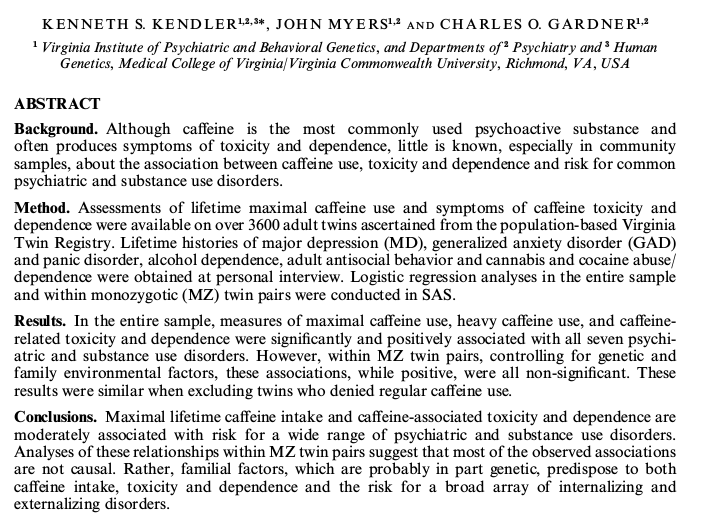
\includegraphics[width=\textwidth]{caffeine-twin-study}

\end{frame}

\section<article>{Summary}
\section<presentation>*{Summary}

\begin{frame}{Summary}
  \begin{enumerate}
      \item We now have two more ways to compare typical measurement values between two samples.
      \item The \alert{sign test} is very flexible, and doesn't even require numeric measurements.
      \item \ldots count how many pairs have $A>B$.
      \item The Wilcoxon signed-rank test requires the distribution of the difference to be symmetric, but is more powerful than the sign test if this is true.
      \item \ldots add the ranks of the pairs with $A>B$.
      \item Both are distribution-free.
  \end{enumerate}
\end{frame}

% homework
\begin{frame}{Homework}
  \begin{center}

  8.4.3

  \vspace{2em}

  8.4.11

  \vspace{2em}

  8.5.4


  \end{center}
\end{frame}


\end{document}





